%% Template for SDP report, adapted from mlp_cw2_template, 2018. 

%% Based on  LaTeX template for ICML 2017 - example_paper.tex at 
%%  https://2017.icml.cc/Conferences/2017/StyleAuthorInstructions

\documentclass{article}
\usepackage[T1]{fontenc}
\usepackage{amssymb,amsmath}
\usepackage{txfonts}
\usepackage{microtype}
\usepackage{xspace}
\xspaceaddexceptions{\%}

% Lists with less spacing between items
\usepackage{paralist}

% For figures
\usepackage{graphicx}
\usepackage{subfig} 

% For citations
\usepackage{natbib}

% For algorithms
\usepackage{algorithm}
\usepackage{algorithmic}

% the hyperref package is used to produce hyperlinks in the
% resulting PDF.  If this breaks your system, please commend out the
% following usepackage line and replace \usepackage{mlp2017} with
% \usepackage[nohyperref]{mlp2017} below.
\usepackage{hyperref}
\usepackage{url}
\urlstyle{same}

% Packages hyperref and algorithmic misbehave sometimes.  We can fix
% this with the following command.
\newcommand{\theHalgorithm}{\arabic{algorithm}}


% Set up MLP coursework style (based on ICML style)
\usepackage{mlp2018}
\mlptitlerunning{SDP Demo \demoNumber  Group (\groupNumber)}
\bibliographystyle{icml2017}


\DeclareMathOperator{\softmax}{softmax}
\DeclareMathOperator{\sigmoid}{sigmoid}
\DeclareMathOperator{\sgn}{sgn}
\DeclareMathOperator{\relu}{relu}
\DeclareMathOperator{\lrelu}{lrelu}
\DeclareMathOperator{\elu}{elu}
\DeclareMathOperator{\selu}{selu}
\DeclareMathOperator{\maxout}{maxout}







%% You probably do not need to change anything above this comment

%% REPLACE the details in the following commands with your details
\setGroupNumber{15}
\setGroupName{Detroit}
\setProductName{Tadashi}
\setDemoNumber{3}
\setLogoFileName{figs/logo-small.png}

\begin{document} 

\makeSDPTitle{Demo}

% Previous MLP Style Title Layout working. 
% \twocolumn[
    % \mlptitle{\productName: SDP Demo \demoNumber}
    % \centerline{Group \groupNumber: \groupName}
% ]

\begin{abstract} 
The abstract should consist of one sentence describing the intended functionality of your system, followed by a few sentences (100--200 words) summarising the key advances made for this demo. This should give the reader a clear expectation of what will be demonstrated.
\end{abstract} 

\section{Project plan update} 

\begin{itemize}
\item Begin testing app with non-technical users to gain insights on accessibility and ease of use: {\bf achieved}.
\item Make changes to app justified against results of testing: {\bf partially achieved}.
\item Complete user interviews with caregivers to assess demand for project features and implement new features based on caregiver requests: {\bf not achieved}.
\item Physically integrate lift mechanism into robot body, and integrate lift control into robot control software: {\bf achieved}.
\item Design and manufacture a tray to place on top of the lift to hold items: {\bf achieved}.
\item Add sensor to lift to determine whether items have been removed: {\bf achieved}.
\item Refine robot problem-solving when stuck by tuning mapping sensitivity and obstacle avoidance logic: {\bf partially achieved}. 
\item Implement bi-directional communication between the app and robot: {\bf achieved}.
\end{itemize}

Concisely summarise the reasons for any deviations from achievement of your intended goals.

Provide a one paragraph description of how your group organised the work towards the goals, including specific indication of which group member worked on which aspect(s). Highlight any methods used to ensure effective group work such as protocols for code integration, task tracking, automated testing, etc.

Provide a summary of how your budget has been spent so far.

Provide a clear statement of any modification (relative to your original plan) that you wish to make to your goals for the next demonstration.

\section{Technical details}

This section should describe in technical terms the current status of your system implementation. It should provide clear justification for any design decisions, with brief reference to any alternatives considered or explored. If your implementation is based on the work of others (e.g. you have found a specific vision processing algorithm) you should cite the source (e.g. \cite{Newell81}) and add the details to the example-refs.bib file so that the full reference appears in the bibliography section. Note you can also refer back to your own previous reports. 

You can export references in the bibtex format from Google Scholar. Click the quotation marks underneath the study name, click 'Bibtex' in the new popup. You can then copy and paste this code into example-refs.bib.

The following are some suggested subsections. You might also want to include a system overview diagram showing how all the relevant parts connect. 

\subsection{Hardware}

Explain any construction on the hardware parts of your system, including choice and placement of sensors and actuators. Pictures should be used if appropriate (for instance, figure~\ref{fig:sample-fig}), using the \verb+\includegraphics+ environment to include an image (pdf, png, or jpg formats), ideally with informative labels added. 

To keep your folders clean, it is often a good idea to keep your images in a separate folder. In this example, we've put the figures in the \texttt{figs/} folder. To include images from different folders, give the relative path from this file. Example: \verb+\includegraphics{figs/image_filename}+.

\begin{figure}[tb]
\vskip 5mm
\begin{center}
\centerline{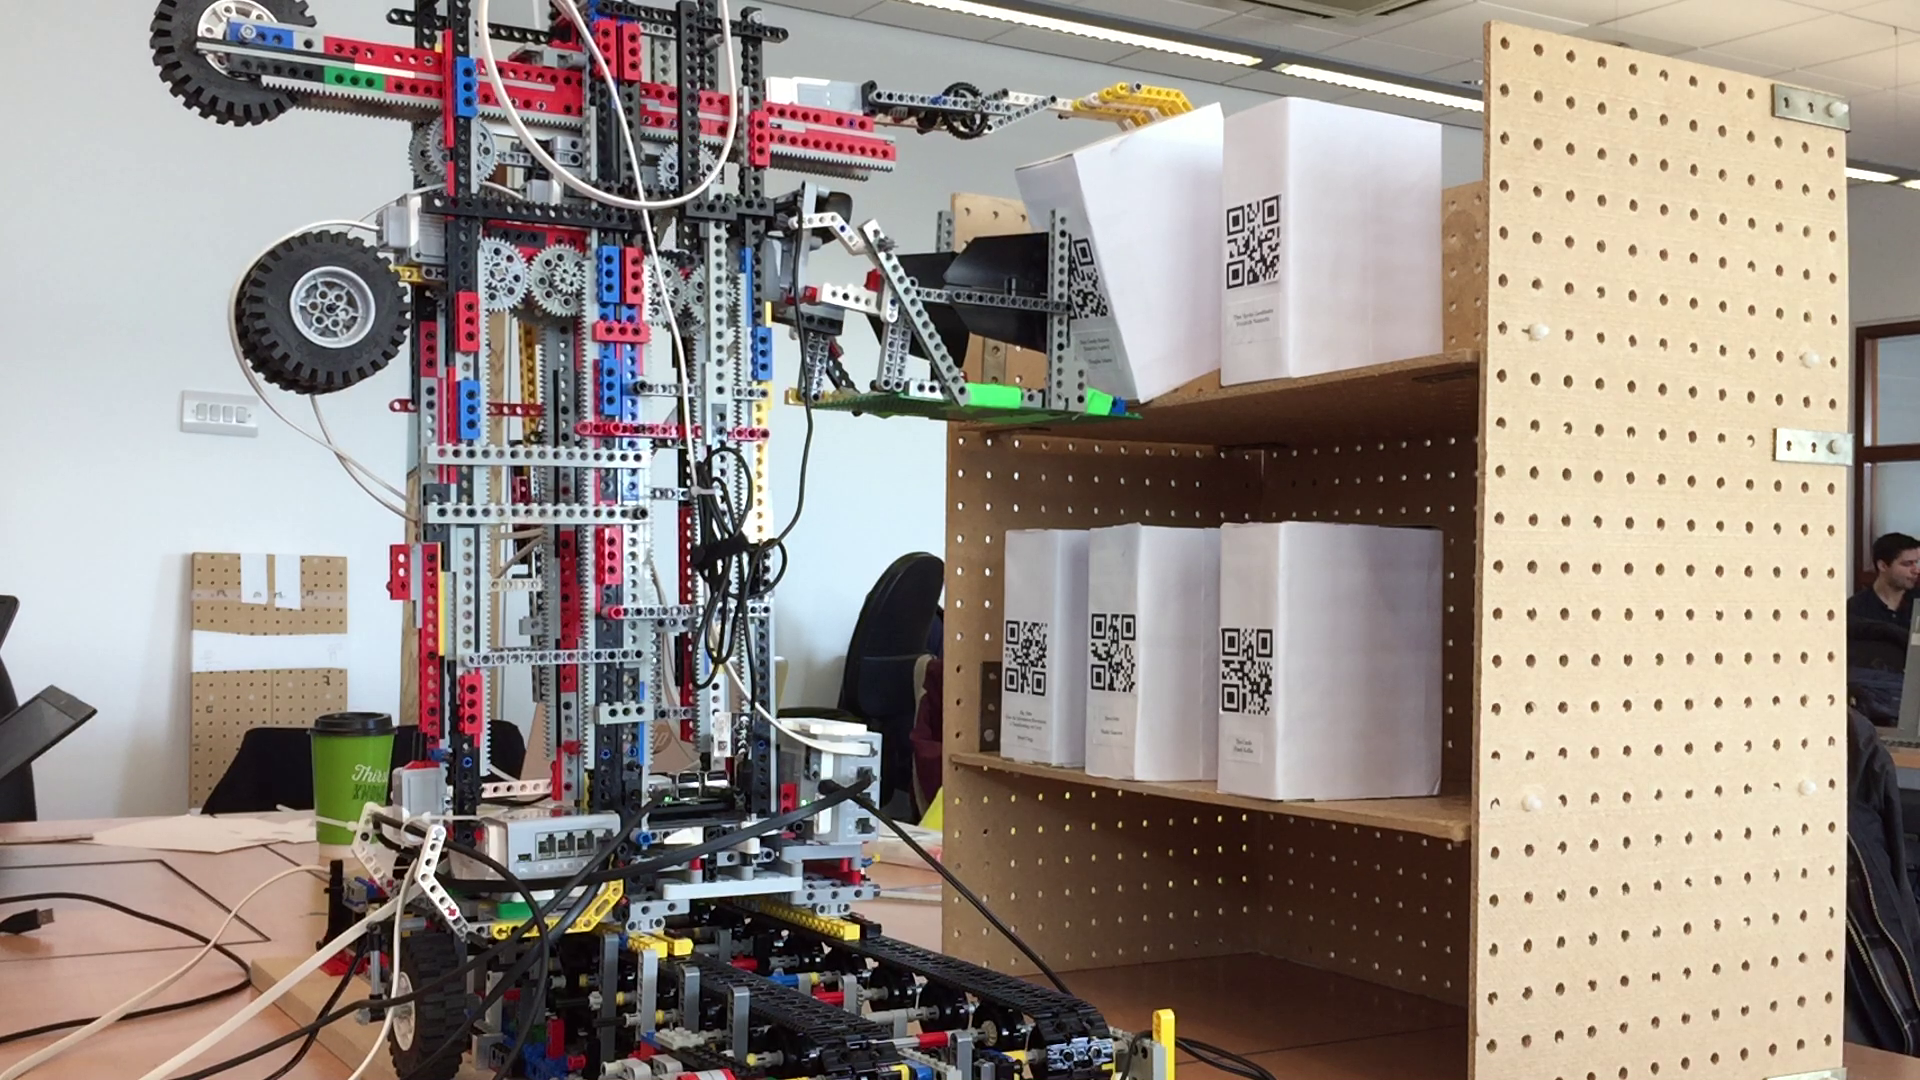
\includegraphics[width=\columnwidth]{figs/crane}}
\caption{Lego construction: highlight any salient features in the caption}
\label{fig:sample-fig}
\end{center}
\vskip -5mm
\end{figure} 

\subsection{User interface}

Depending on your system and its stage of development, it could be useful to include a section about the user interface design, and the usability decisions behind it. Note, however, that you will be asked to provide a separate 'user guide' for the final demo.

\subsection{Software}

From its state in the previous demo, the robot software has moved towards what would have been our envisaged final product. In summary, it has evolved in the following key ways:

\begin{itemize}
  \item The robot now keeps track of a variety of variables regarding its state
  \item The robot now calculates a vector to its intended destination from its current position rather than using hardcoded distances on x and y
  \item The robot can now control the lift directly through a serial connection between the Raspberry Pi board and the arduino controlling the lift
  \item The ROS node controlling the navigation stack and networking is now able to communicate with the app bidirectionally
  \item The parameters powering the robots autonomous navigation have been configured in order to suit our configuration more appropriately
\end{itemize}

For obvious reasons, we wanted the app to be able to access certain information about the current state of our robot. The information we decided would be particularly important is the state of its battery, as well as its current 'behaviour'. These different status' are stored in a dictionary. We decided to use a dictionary over a list so that we could assign our own code to each state. This would be useful later on if we were to implement some kind of error recognition i.e. \it{def a} should not run if the state is less than 0. We note that in the average case, item retreival is O(1) in both lists and dictionaries and so there was no obvious reason against using a dictionary here given this is all we use ours for. The states we had included at this stage were: low battery, assistance required, at base/not busy, moving, and arrived at goal.

% Explain the key details of the control and interface software developed for the project. Be clear about any packages used and the reason for choosing them. 

% If you present algorithms, you can use the \verb+algorithm+ and \verb+algorithmic+ environments to format pseudocode (for instance, Algorithm~\ref{alg:example}). These require the corresponding style files, \verb+algorithm.sty+ and \verb+algorithmic.sty+ which are supplied with this package. 

% \begin{algorithm}[ht]
% \begin{algorithmic}
%    \STATE {\bfseries Input:} data $x_i$, size $m$
%    \REPEAT
%    \STATE Initialize $noChange = true$.
%    \FOR{$i=1$ {\bfseries to} $m-1$}
%    \IF{$x_i > x_{i+1}$} 
%    \STATE Swap $x_i$ and $x_{i+1}$
%    \STATE $noChange = false$
%    \ENDIF
%    \ENDFOR
%    \UNTIL{$noChange$ is $true$}
% \end{algorithmic}
%   \caption{Bubble Sort}
%   \label{alg:example}
% \end{algorithm}

\section{Evaluation}

This section should first outline any testing methods you used (e.g. repeated runs of subsystems, data-logging, naive user testing). 

It should then present relevant quantitative results. If you are using graphs, please make sure they are properly labelled and logically illustrate the point you want to make (e.g. to compare two algorithms).


At an absolute minimum, this section should provide a table (for instance, table~\ref{tab:sample-table}, using the \verb+table+ environment) of success rates for repeated runs of the whole system (as you will only be able to show one run in the demo).

\begin{table}[h]
\vskip 3mm
\begin{center}
\begin{small}
\begin{sc}
\begin{tabular}{lcccr}
\hline
\abovespace\belowspace
Test  & Time(mins) & Errors & Success \\
\hline
\abovespace
1    & 1:30 & 0 & $\surd$ \\
2    & 3:00 & 2 & $\times$\\
3    & 2:20 & 1 & $\surd$ \\
4    & 1:50 & 1 & $\times$\\
\belowspace
5    & 2:10 & 0 & $\surd$ \\
\hline
\end{tabular}
\end{sc}
\end{small}
\caption{Results for 5 tests of the system.}
\label{tab:sample-table}
\end{center}
\vskip -3mm
\end{table}

If you need a figure or table to stretch across two columns use the \verb+figure*+ or \verb+table*+ environment instead of the \verb+figure+ or \verb+table+ environment.  Use the \verb+subfigure+ environment if you want to include multiple graphics in a single figure.

\section{Budget}
\begin{table}[h]
\begin{center}
    \resizebox{\columnwidth}{!}{
  \begin{tabular}{lllll}
    {\bf Item} & {\bf Units} & {\bf Cost (\pounds\ per unit)} & {\bf Total cost (\pounds)} & {\bf Use} \\
    \hline
    Turtlebot Waffle & 1 & 1275.80 & 1275.80 & Robot \\
    Lego & 2.5kg & 15.00 & 37.50 & Lift \\
    \hline \hline
               &       & Overall cost (\pounds) & 1787.43
  \end{tabular}}
\caption{Non-budgeted monetary costs at demo \demoNumber.}
\label{tab:non-budget-cost}
\end{center}
\end{table}

\begin{table}[h]
\begin{center}
  \resizebox{\columnwidth}{!}{
  \begin{tabular}{lllll}
    {\bf Item} & {\bf Total cost (\pounds)} & {\bf Use} \\
    \hline
    Turtlebot supports  & 8.00 & Lift \\
    MDF support (12mm x 270mm x 400mm) & 1.00  & Lift \\
    Lift support rods & 5.00 & Lift \\
    Pegboard ($0.62 \text{m}^2$ at \pounds 12 per $2.88 \text{m}^2$)& 2.59 & Arena \\
    Misc (wires, screws, angle brackets) & 5.00 & Lift, arena \\
    \hline
    \hline
     Budget spent (\pounds) & 21.59 \\
     Budget remaining (\pounds) & 178.41   
  \end{tabular}}
\caption{Budgeted monetary costs at demo \demoNumber. MDF value is approximate as 12mm MDF is not on the SDP price sheet.}
\label{tab:budget-cost-monetary}
\end{center}
\end{table}

\begin{table}[h]
\begin{center}
  \resizebox{\columnwidth}{!}{
  \begin{tabular}{lll}
    {\bf Purpose} & {\bf Hours spent} & {\bf Use} \\
    \hline
    Manufacturing lift support rods & 1 & Lift \\
    Manufacturing lift base (MDF) & 0.5 & Lift \\
    Drilling holes in lift base & 0.25 & Lift \\
    \hline
    \hline
    Overall technician hours spent & 1.75 & \\
    Total technician hours remaining & 5.25
  \end{tabular}}
\caption{Budgeted technician time at demo \demoNumber. Note that hours remaining includes subtracting any hours lost due to not being used in previous weeks.}
\label{tab:budget-cost-non-monetary}
\end{center}
\end{table}


%% Include any references in a bibliography

\bibliography{example-refs}

\end{document} 

